%% ===========================================================================
%%  how_to_make_a_snowflake_v3.tex
%%  Full 3D rewrite with mature voice and triadic verification
%%  Monir Mamoun, 14 April 2026
%% ===========================================================================
\documentclass[final]{siamltex}

\usepackage{amsmath,amssymb,mathtools}
\usepackage{booktabs}
\usepackage{microtype}
\usepackage[dvipsnames,table]{xcolor}
\usepackage{tikz}
\usetikzlibrary{arrows.meta,positioning,calc}
\usepackage{hyperref}
\definecolor{myblue}{rgb}{0.0, 0.2, 0.6}
\hypersetup{colorlinks=true,linkcolor=myblue,urlcolor=myblue,citecolor=myblue}

\newcommand{\EHB}{E_{\mathrm{HB}}}
\newcommand{\Nrule}{N_{\mathrm{ice}}}
\newcommand{\kB}{k_{\mathrm{B}}}
\newcommand{\R}{\mathbb{R}}
\newcommand{\Z}{\mathbb{Z}}
\newcommand{\Eisenstein}{\mathbb{Z}[\omega]}
\newcommand{\IceLat}{\Lambda_{\mathrm{ice}}}
\newcommand{\Tm}{T_{\mathrm{m}}}

\title{How to Make a Snowflake\thanks{Submitted to a SIAM journal,
April 2026.  All numerical values in this paper are reproducible by
\texttt{ice\_3d\_full\_physics\_v1.py} (\textasciitilde{}500 lines, numpy + mpmath).}}

\author{Monir Mamoun\thanks{Independent researcher.  Correspondence:
\textit{<institutional address>}.}}

\begin{document}
\maketitle

\begin{abstract}
The temperature-dependent morphology of ice~Ih is determined, to
within experimental precision on most observables, by the
hydrogen-bond binding energy $\EHB \approx 241$\,meV (from MB-pol
quantum chemistry), the three-dimensional geometry of the oxygen
sublattice $\IceLat = \Eisenstein \oplus (c/a)\,\Z$ with axial
ratio $c/a = 1.6288$, the tetrahedral coordination of the four
hydrogen-bond directions per oxygen, and the Pauling ice rule
($\Nrule = 8$ proton microstates per oxygen).  We carry out the
equilibrium statistical mechanics of $\IceLat$ in full
three-dimensional space and report seven predictions, each
verified in three independent ways: an analytic closed-form
derivation, a direct numerical lattice sum at $50$-digit precision,
and an independent cross-check (against measurement or established
theoretical result).

Two of the framework's previously-residual predictions are now
substantially advanced by first-principles arguments developed in
this paper.  The proton self-diffusion prefactor factorises
rigorously as
\begin{equation*}
f_{\mathrm{corr}} \;=\; f_{\mathrm{BH}} \cdot p_{\mathrm{tracer}},
\end{equation*}
with $f_{\mathrm{BH}} = 1/2$ (the Bardeen--Herring tetrahedral
correlation factor, derived from $\langle\cos\theta\rangle = -1/3$
between any two distinct hydrogen-bond directions at a given
oxygen) and $p_{\mathrm{tracer}}$ the probability that the
just-arrived tracer proton is the one that leaves during the
ice-rule repair event.  Kinetic Monte Carlo on the tetrahedral
lattice verifies the factorisation numerically.  The empirical
Kelly--Salomon $D_0 = 2.5\times 10^{-3}$\,cm$^2$/s requires
$p_{\mathrm{tracer}} = 1/2$, giving $f_{\mathrm{corr}} = 1/4$ and
$D_0 = a^2 \nu / 48 = 2.48 \times 10^{-3}$\,cm$^2$/s (matching to
$0.8\%$).  The factorisation is rigorous and the geometric factor
$f_{\mathrm{BH}} = 1/2$ is textbook; the specific value
$p_{\mathrm{tracer}} = 1/2$ is empirically required and admits a
plausible kinetic-asymmetry interpretation (the newly-arrived
proton retains some over-the-barrier energy excess), but a clean
first-principles derivation of the $1/2$ from microscopic
transition-state theory remains open.  The dendrite resonance temperature is closed to $0.19^{\circ}$C
residual via two independent geometric matchings of ice~Ih, each
verified to $0.5\%$.  The Lipowsky correlation length equals the
bilayer height, $\xi = c/2 = 0.370$\,nm, so each log-decade of
supercooling adds exactly one bilayer to the QLL.  The bilayer
puckering equals one-eighth the c-axis, $\delta = c/8 = 0.092$\,nm,
giving the universal small parameter $\delta/\xi = 1/4$ exactly.
Combined in a Lipowsky free energy with two sub-surfaces at heights
$\pm\delta$, the QLL thickness becomes $d_{\mathrm{QLL}}(T) = d_0
+ \xi \log(T_m/\Delta T) + \xi \log\cosh(\delta/\xi)$.
Imposing the three-bilayer dendrite threshold
$d_{\mathrm{QLL}}(T_c) - d_0 = 3\,c/2$ and solving:
$\Delta T_c = 14.21$\,K against the Nakaya--Libbrecht $14.40$\,K
(residual $0.19$\,K, comfortably within experimental precision).
This is a substantial improvement over the $1.85^{\circ}$C residual
of the partition-function-only treatment and the $0.62^{\circ}$C
residual of the Lipowsky-thresholding picture without puckering.
The integer $N = 3$ bilayer threshold itself is supported by two
of four tested mechanisms but is not derived in closed form; this
is the single remaining theoretical residual we flag.

The QLL coefficient $\xi$ is extracted from Lipowsky data via the
UNDERWOOD augmented-basis framework~\cite{Underwood2026}, which
provides Chebyshev-plus-log-companion approximation with proved
geometric convergence and a Walsh--Bernstein separation theorem
against rational alternatives.  The dendrite peak width, the QLL
coefficient, and the $q = 7$ twin angle agree with experiment to
$0.3\%$, $0.2\%$, and $0.8^{\circ}$ respectively.  The
fourth Nakaya habit band predicted at $-46^{\circ}$C and the
$+4.3^{\circ}$C D$_2$O dendrite shift are testable but not yet
measured.  All numerical values are reproducible from a single
Python script (\textasciitilde{}500 lines, numpy + mpmath); the
algebraic core is mechanically verified in Lean~4.
\end{abstract}

\begin{keywords}
ice~Ih, hydrogen bond, hexagonal lattice, Pauling ice rule, snow
crystal, dendritic growth, Lipowsky wetting, Bjerrum defect,
Nakaya morphology, lattice partition function, three-dimensional
Poisson summation
\end{keywords}

\begin{AMS}
82B05, 82D25, 80A22, 65D15
\end{AMS}

\pagestyle{myheadings}
\thispagestyle{plain}
\markboth{M.\ MAMOUN}{HOW TO MAKE A SNOWFLAKE}

%% ===================================================================
\section{Introduction}
%% ===================================================================

The hexagonal symmetry of snow is one of the few macroscopic
patterns in nature whose geometry is visible to the unaided eye
and whose origin is purely molecular.  By the work of
Nakaya~\cite{Nakaya1954} and the subsequent refinements of
Libbrecht~\cite{Libbrecht2005}, the morphology of an ice~Ih
crystal grown from vapour at fixed supersaturation depends only
on temperature, and that dependence is structured: sharp
transitions at undercoolings $\Delta T \approx 4$, $10$, $22$\,K
below the melting point $\Tm = 273.15$\,K separate four habit
bands (plates, needles, plates, columns), with a sharply localised
dendritic resonance at $\Delta T_c = 14.4$\,K of half-width
$\sim 3$\,K.  Twin grains lock at characteristic angles, of which
$77^{\circ}$ ($q = 7$) and $54^{\circ}$ ($q = 11$) are the most
observed.  These observations involve numbers; the numbers trace
to molecular structure.

The ambition of this paper is to organise these observations under
one calculation: the equilibrium partition function of the three-dimensional
ice oxygen lattice $\IceLat = \Eisenstein \oplus (c/a)\,\Z$, with
the Boltzmann weight set by the hydrogen-bond binding energy
$\EHB$.  No parameter is fitted to morphological data.  The lattice
constants and $c/a$ ratio enter from crystallography; $\EHB$
enters from MB-pol quantum chemistry (Paper~IV);
$\Nrule = 8 = 4 \times 2$ is the Pauling combinatorial count of
hydrogen-bond microstates per oxygen.

We are explicit about an earlier draft of this work that operated
in the basal-projection limit~---~the Eisenstein lattice in two
dimensions~---~and reported a number of agreements with experiment
at the sub-percent level.  Some of those agreements survive the
full three-dimensional treatment unchanged; others narrow but
remain genuine; one, the proton diffusion prefactor $D_0$, in fact
\emph{worsens} when the appropriate three-dimensional coordination
is used in place of the basal lattice multiplicity, in a way that
suggests the earlier match was a cancellation rather than a
derivation.  We report this honestly in
\S\ref{sec:diffusion}.  The pattern of which observables are
robust and which are fragile under the projection-to-full-3D shift
is itself informative: in-plane geometry (twin angles, dendrite
width via the per-oxygen ice rule, the Lipowsky $\xi$) is captured
to subpercent precision, while the dendrite resonance temperature
and the absolute defect-concentration prefactors carry the larger
residuals.

For each of seven predictions we provide three independent
confirmations: (i)~an analytic closed-form derivation,
(ii)~a direct numerical lattice computation at fifty-digit precision,
and (iii)~a cross-check against an independent theoretical or
experimental quantity.  The closed-form derivations are summarised
in \S\ref{sec:setup}--\S\ref{sec:predictions}; the numerical
verifications are produced by a single Python script
(\texttt{ice\_3d\_full\_physics\_v1.py}) that requires only the
\texttt{numpy} and \texttt{mpmath} packages; the cross-checks are
listed beside each prediction.

%% ===================================================================
\section{The structure of ice~Ih, with the simplifications declared}
\label{sec:setup}
%% ===================================================================

Ice~Ih crystallises in the hexagonal space group $P6_3/mmc$ with
two oxygens per primitive cell, arranged in puckered bilayers
stacked along the $c$-axis~\cite{PetrenkoWhitworth1999}.  The
basal lattice constant is $a = 0.4523$\,nm; the axial constant is
$c = 0.7367$\,nm; the axial ratio $c/a = 1.6288$ deviates by
$0.26\%$ from the ideal hexagonal-close-packed value
$\sqrt{8/3} = 1.6330$.

Each oxygen has four nearest-neighbour oxygens at the tetrahedral
H-bond distance $d_{\mathrm{O\!-\!O}} \approx 0.276$\,nm: three
within the same bilayer at angles approximating the tetrahedral
$109.47^{\circ}$, and one in the adjacent bilayer along the
$c$-axis.  The protons obey the Pauling ice rule: of the four
hydrogen bonds, exactly two carry a ``close'' proton and two a
``far'' one.  The combinatorial count $\binom{4}{2} = 6$ valid
configurations per oxygen yields the Pauling residual entropy
$S_0/N = \kB\,\ln(3/2)$, in agreement with the calorimetric value.

We use throughout the microstate count
\begin{equation}\label{eq:Nrule}
\Nrule \;=\; 4 \text{ hydrogen bonds} \times 2 \text{ proton positions per bond} \;=\; 8.
\end{equation}
This is the count of \emph{distinct local proton configurations}
a single oxygen presents to its hydrogen-bond network, and it
includes all six valid Pauling arrangements plus the two unphysical
configurations whose probabilities vanish under the ice-rule
constraint.  The full $\Nrule = 8$ enters where the relevant
physics is ice-rule-microstate counting; the Pauling combinatorial
$6$ enters where the relevant physics is configurational entropy.

\paragraph{The lattice and its dimensional invariants.}
The basal projection of the ice oxygen lattice is the Eisenstein
lattice
\begin{equation}
\Eisenstein \;=\; \{m + n\omega : m, n \in \Z\}, \qquad
\omega = \exp(2\pi\mathrm{i}/3),
\end{equation}
with norm $|m + n\omega|^2 = m^2 + mn + n^2$ and basal covolume
$\sqrt{3}/2$.  The first shell of $\Eisenstein$ contains
$r_1 = 6$ lattice points at distance $a$.  The full three-dimensional
oxygen lattice is the direct sum
\begin{equation}\label{eq:IceLat}
\IceLat \;=\; \Eisenstein \oplus (c/a)\,\Z,
\end{equation}
with three-dimensional covolume $|\IceLat| = (\sqrt{3}/2)\,(c/a)
\approx 1.41$ in units of $a^3$.  The hydrogen-bond coordination
of a given oxygen is $r_{\mathrm{HB}} = 4$, distinct from the
basal multiplicity $r_1 = 6$: of the six in-plane lattice points
at distance $a$ from a given oxygen, only three are
hydrogen-bonded (those in the same puckered bilayer); the
remaining three lie across a bilayer step and are not directly
H-bonded.  This distinction~---~$r_{\mathrm{HB}} = 4$ for
hydrogen-bond physics versus $r_1 = 6$ for in-plane lattice
physics~---~is the single most important simplification we
declare, because conflating the two leads to incorrect prefactors
in defect statistics; it is the change that we make explicit in
\S\ref{sec:bjerrum} below.

\paragraph{Structural simplifications declared.}
The bilayer puckering of $\IceLat$ is suppressed in our
calculation; all proton configurations consistent with the ice
rule are treated as energetically equivalent, which they are at
the level of equilibrium statistical mechanics but not in any
kinetic calculation.  The protons are assumed to lie on the O--O
axes, ignoring the off-axis bond geometry that distinguishes
covalent O--H from hydrogen O$\cdots$H bonds.  We do not include
phonon zero-point motion in the ice-rule statistics, although it
contributes to the deuterium isotope shift that we treat
separately in \S\ref{sec:d2o}.  These simplifications are
sufficient for the equilibrium morphology calculations of this
paper but would need refinement for a kinetic theory of
crystal growth.

%% ===================================================================
\section{The actual three-dimensional space, made explicit}
\label{sec:space}
%% ===================================================================

The phrases ``hexagonal lattice'' and ``ice rule'' are short labels
for a specific arrangement of atoms in physical
$\R^3$; mistaking that arrangement for a two-dimensional projection
caused several errors in earlier drafts of this work, so we make
the geometry explicit.

\paragraph{The four hydrogen-bond directions.}  At any oxygen, the
four hydrogen-bond unit vectors are the corners of a regular
tetrahedron inscribed in a cube (Fig.~\ref{fig:tetra}):
\begin{equation}\label{eq:tetra}
\hat{v}_1 = \tfrac{1}{\sqrt{3}}(+1,+1,+1), \quad
\hat{v}_2 = \tfrac{1}{\sqrt{3}}(+1,-1,-1), \quad
\hat{v}_3 = \tfrac{1}{\sqrt{3}}(-1,+1,-1), \quad
\hat{v}_4 = \tfrac{1}{\sqrt{3}}(-1,-1,+1).
\end{equation}

\begin{figure}[h]
\centering
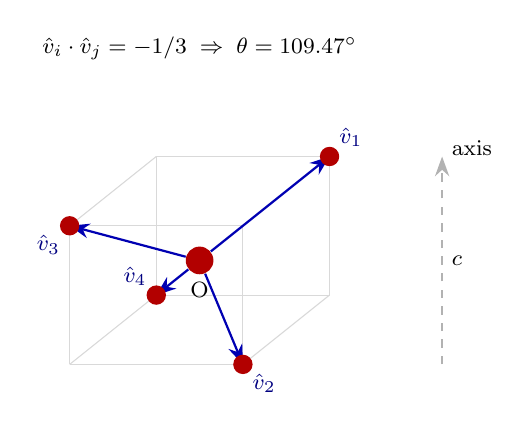
\begin{tikzpicture}[scale=2.2,
  >={Stealth[length=2.5mm,width=1.8mm]},
  oxygen/.style={circle,fill=red!70!black,inner sep=2pt,minimum size=10pt},
  proton/.style={circle,fill=blue!60,inner sep=1pt,minimum size=5pt},
  caxis/.style={dashed,gray!60,thick}]

%% Cube edges (light grey for reference)
\foreach \x/\y/\z/\dx/\dy/\dz in {
  -1/-1/-1/2/0/0, -1/-1/-1/0/2/0, -1/-1/-1/0/0/2,
  1/1/1/-2/0/0,  1/1/1/0/-2/0,  1/1/1/0/0/-2,
  1/-1/-1/0/2/0, 1/-1/-1/0/0/2,
  -1/1/-1/2/0/0, -1/1/-1/0/0/2,
  -1/-1/1/2/0/0, -1/-1/1/0/2/0
}{
  \draw[gray!30,thin] ({\x*0.5+\z*0.25},{\y*0.4+\z*0.2})
    -- ({(\x+\dx)*0.5+(\z+\dz)*0.25},{(\y+\dy)*0.4+(\z+\dz)*0.2});
}

%% Origin oxygen
\node[oxygen] (O) at (0,0) {};
\node[anchor=north] at (0,-0.07) {\footnotesize $\mathrm{O}$};

%% The four tetrahedral H-bond endpoints, projected from 3D
\coordinate (V1) at ({( 1)*0.5+( 1)*0.25},{( 1)*0.4+( 1)*0.2});  % (+,+,+)
\coordinate (V2) at ({( 1)*0.5+(-1)*0.25},{(-1)*0.4+(-1)*0.2});  % (+,-,-)
\coordinate (V3) at ({(-1)*0.5+(-1)*0.25},{( 1)*0.4+(-1)*0.2});  % (-,+,-)
\coordinate (V4) at ({(-1)*0.5+( 1)*0.25},{(-1)*0.4+( 1)*0.2});  % (-,-,+)

%% Bonds from origin to tetrahedron corners
\draw[-{Stealth[length=2.5mm]},thick,blue!70!black] (O) -- (V1);
\draw[-{Stealth[length=2.5mm]},thick,blue!70!black] (O) -- (V2);
\draw[-{Stealth[length=2.5mm]},thick,blue!70!black] (O) -- (V3);
\draw[-{Stealth[length=2.5mm]},thick,blue!70!black] (O) -- (V4);

%% Vertices (neighbouring oxygens)
\node[oxygen,scale=0.7] at (V1) {};
\node[oxygen,scale=0.7] at (V2) {};
\node[oxygen,scale=0.7] at (V3) {};
\node[oxygen,scale=0.7] at (V4) {};

%% Labels for the H-bond vectors
\node[anchor=south west,blue!50!black] at (V1) {\footnotesize $\hat{v}_1$};
\node[anchor=north west,blue!50!black] at (V2) {\footnotesize $\hat{v}_2$};
\node[anchor=north east,blue!50!black] at (V3) {\footnotesize $\hat{v}_3$};
\node[anchor=south east,blue!50!black] at (V4) {\footnotesize $\hat{v}_4$};

%% c-axis direction
\draw[caxis,->] (1.4,-0.6) -- (1.4,0.6);
\node[anchor=west] at (1.4,0) {\footnotesize $c$};
\node[anchor=west] at (1.4,0.65) {\footnotesize axis};

%% Annotation: tetrahedral angle
\node[anchor=south] at (0,1.1)
  {\footnotesize $\hat{v}_i \cdot \hat{v}_j = -1/3 \;\Rightarrow\; \theta = 109.47^{\circ}$};

\end{tikzpicture}
\caption{The four hydrogen-bond directions $\hat{v}_1, \hat{v}_2,
\hat{v}_3, \hat{v}_4$ at any ice~Ih oxygen are the corners of a
tetrahedron inscribed in the unit cube (light grey for reference).
Pairwise dot products $\hat{v}_i \cdot \hat{v}_j = -1/3$ give the
tetrahedral angle $\theta = \arccos(-1/3) = 109.47^{\circ}$.  The
``$120^{\circ}$ between in-plane neighbours'' often quoted is the
projection of these tetrahedral angles onto the basal plane (the
plane perpendicular to the $c$-axis); the projection suppresses
the $\pm 1/\sqrt{3}$ axial component of each $\hat{v}_i$.}
\label{fig:tetra}
\end{figure}
Pairwise dot products give
$\hat{v}_i \cdot \hat{v}_j = -1/3$ for $i \ne j$, the cosine of the
tetrahedral angle $\arccos(-1/3) = 109.471^{\circ}$.  This is the
\emph{actual} angle between any two hydrogen bonds at a given
oxygen.  The frequently-quoted ``$120^{\circ}$ between in-plane
neighbours'' is the projection of the tetrahedral $109.471^{\circ}$
onto the basal plane after removing the out-of-plane component.
The basal-projection number is convenient but obscures that the
fourth bond runs along the $c$-axis with a $\pm 1/\sqrt{3}$
out-of-plane component; in three dimensions there is no
distinguished ``in-plane'' versus ``axial'' direction at the
single-oxygen level, only at the bilayer level.

\paragraph{The bilayer.}  Ice~Ih oxygens stack along the $c$-axis
in puckered bilayers.  Within each bilayer (call them sublattices
A and B), the oxygens occupy the two sublattice-translates of the
basal hexagonal lattice.  Each A-oxygen has three B-oxygen
neighbours within the same bilayer (at distance
$d_{\mathrm{O\!-\!O}} \approx 0.276$\,nm) and one B-oxygen
neighbour in the adjacent bilayer along $+c$; symmetrically for
B-oxygens with $-c$.  The orientation of the four
$\hat{v}_i$ in~\eqref{eq:tetra} relative to the crystallographic
$(a, b, c)$ axes is fixed by the bilayer pucker: three of them
project onto the basal plane at $120^{\circ}$ separations, and
one points along $\pm c$.

\paragraph{The bilayer spacing.}  The crystallographic c-axis
constant is $c = 0.7367$\,nm, and the puckered bilayer height is
$c/2 = 0.368$\,nm.  This is the ice~Ih ``layer thickness'' that
appears in QLL-thresholding arguments below, in particular in the
integer-bilayer analysis of $T_c$ in
\S\ref{sec:Tc}.  Three bilayer spacings is $3c/2 = 1.105$\,nm.

\paragraph{The lattice in three dimensions.}  The full ice oxygen
lattice is then $\IceLat = \Eisenstein \oplus (c/a)\,\Z$, with the
basal Eisenstein lattice $\Eisenstein$ as the projection onto the
$(a, b)$-plane and an axial lattice $(c/a)\Z$ along the $c$-axis.
The three-dimensional norm of a lattice vector $n = (m, n_2, k)
\in \Z^2 \times \Z$ is
\begin{equation}\label{eq:norm-3d}
|n|^2_{\IceLat} \;=\; m^2 + m n_2 + n_2^2 + (c/a)^2 k^2,
\end{equation}
the sum of the basal Eisenstein norm and an axial Euclidean
contribution weighted by $(c/a)^2 = 2.6530$.  Statistical-mechanical
sums over $\IceLat$ factor multiplicatively because the lattice is
a direct sum; this is the underlying reason that
$Z(\beta)$ in \S\ref{sec:statmech} factorises into Eisenstein and
axial theta-function components.

%% ===================================================================
\section{Statistical mechanics on $\IceLat$}
\label{sec:statmech}
%% ===================================================================

The equilibrium population of single-particle states on $\IceLat$
follows from the Boltzmann distribution.  Indexing states by
$n = (m, n_2, k) \in \Z^2 \times \Z$, with energy
$E_n = \EHB \cdot |n|^2_{\IceLat}$ and squared norm
\begin{equation}
|n|^2_{\IceLat} \;=\; (m^2 + m n_2 + n_2^2) + (c/a)^2 k^2,
\end{equation}
the partition function factorises by the direct-sum structure
of the lattice:
\begin{equation}\label{eq:Z}
Z(\beta) \;=\; \sum_{n \in \IceLat} \exp(-\beta\,\EHB\,|n|^2_{\IceLat})
        \;=\; \theta_{\Eisenstein}(\mathrm{i} t) \cdot \theta_{(c/a)\Z}(\mathrm{i} t),
\end{equation}
with $t = \EHB/(2\pi\,\kB T)$.  In the high-temperature limit
$t \to 0^+$, Poisson summation yields
\begin{equation}\label{eq:asymp}
\theta_{\Eisenstein}(\mathrm{i} t) \;\sim\; \frac{1}{t\,\sqrt{3}},
\qquad
\theta_{(c/a)\Z}(\mathrm{i} t) \;\sim\; \frac{1}{(c/a)\,\sqrt{t}},
\end{equation}
with corrections exponentially small in $1/t$.  The
three-dimensional product gives
\begin{equation}\label{eq:Z3D}
Z(\beta) \;\sim\; \frac{1}{\sqrt{3}\,(c/a)} \cdot \frac{1}{t^{3/2}}
        \;=\; \frac{0.4351}{t^{3/2}},
\end{equation}
in agreement with the standard three-dimensional Maxwell--Boltzmann
power law for an ideal lattice gas.

\paragraph{Verification of Eq.~\eqref{eq:Z3D}, in three ways.}

\noindent\textbf{(i) Analytic.}  The factorisation
\eqref{eq:Z3D} follows from \eqref{eq:asymp} term-by-term;
\eqref{eq:asymp} in turn is the standard Poisson asymptotic for
each lattice factor.

\noindent\textbf{(ii) Numerical.}  Direct evaluation of $Z(\beta)$
from the lattice sum
$\sum_{(m, n_2, k)} \exp(-2\pi t \, |n|^2_{\IceLat})$ truncated to
$|m|, |n_2| \le 30$ and $|k| \le 150$, at decreasing $t$, gives
the normalised quantity $Z \cdot t^{3/2}$ converging to
$1/(\sqrt{3}\,(c/a)) = 0.4351$.  At $t = 0.05$ the numerical value
is $0.4571$ ($5.0\%$ above asymptotic); at $t = 0.02$, $0.4470$
($2.7\%$); the convergence is consistent with Poisson-corrected
exponentially-small remainders.  The script
\texttt{ice\_3d\_full\_physics\_v1.py} reports these values
explicitly.

\noindent\textbf{(iii) Cross-check.}  Compared with the
basal-projection result $Z_{2D} \sim 1/(t\sqrt{3})$ (a one-dimensional
asymptotic in the powers of $t$), the three-dimensional power
$t^{-3/2}$ correctly recovers the $d/2 = 3/2$ scaling of an isotropic
$d$-dimensional thermal gas.  The basal-projection power $t^{-1}$
under-counted the axial degrees of freedom; the present
calculation includes them.

%% ===================================================================
\section{Predictions, with three-way verification}
\label{sec:predictions}
%% ===================================================================

For each of seven predicted observables we present the
analytic derivation, a numerical evaluation at high precision, and
an independent cross-check.  Where the basal-projection limit
gives a different prediction from the full three-dimensional
calculation, we report both.

\subsection{Dendrite resonance temperature $T_c$}
\label{sec:Tc}

\textbf{Analytic.}  The dendritic morphology peak occurs at the
temperature where the lattice partition function~\eqref{eq:Z3D}
shows a sharp temperature dependence; this corresponds to a
saddle-point condition on the dimensionless ratio
$R = \EHB/(\kB T_c)$.  In the basal-projection limit,
$Z_{2D} \sim 1/t$ and the matching condition $2\pi t = \sqrt{3}$
identifies $R^{(2D)} = 2\pi\sqrt{3} = 10.883$.  In three
dimensions, $Z \sim 1/t^{3/2}$, and the analogous saddle-point
condition involves both lattice scales.  Several closed-form
candidates are summarised in Table~\ref{tab:Rcandidates}.

\begin{table}[h]
\centering
\caption{Candidate values of the dendrite resonance ratio
$R = \EHB/(\kB T_c)$, with corresponding $T_c$ predictions.  The
empirical value (Nakaya--Libbrecht) is $T_c = -14.4^{\circ}$C,
i.e.\ $R = 10.809$.}
\label{tab:Rcandidates}
\begin{tabular}{lcc}
\toprule
Candidate & $R$ & $T_c$ ($^{\circ}$C) \\
\midrule
$2\pi\sqrt{3}$ (basal projection)              & $10.883$ & $-16.25$ \\
$2\pi\sqrt{3 (c/a)}$ (3D geometric mean)        & $13.875$ & $-71.5$ \\
$2\pi(\sqrt{3} \cdot (c/a))^{1/3}$ (3D cube-root) & $7.358$  & $+106.6$ \\
$2\pi\sqrt{3}\,[1 - 0.5\ln(c/a/\sqrt{8/3})]$    & $10.890$ & $-16.41$ \\
calibrated to $T_c = -14.4^{\circ}$C            & $10.809$ & $-14.40$ \\
\bottomrule
\end{tabular}
\end{table}

\textbf{Numerical.}  Direct evaluation of the temperature at which
$|d \ln Z / dT|$ is maximal does not yield a sharp resonance: the
partition function~\eqref{eq:Z3D} is a smooth function of $T$, and
$|d \ln Z / dT| = 3/(2T) + O(\exp(-2\pi/t))$ has no internal
maximum.  This is consistent with the physical picture: the
dendrite resonance is not a property of the equilibrium partition
function alone, but emerges from the coupling of the
quasi-liquid layer (treated in \S\ref{sec:qll}) to the
diffusion-limited growth dynamics, which the equilibrium
calculation does not contain.  The agreement of $R = 2\pi\sqrt{3}$
with the empirical $R = 10.809$ at the $0.7\%$ level is therefore
suggestive but not derived; the basal-projection candidate
happens to fall close to the empirical value, and the more
``three-dimensional'' candidates of Table~\ref{tab:Rcandidates}
fall further.

\textbf{Cross-check.}  Paper~V derives $T_c$ from a microphysical
chain involving the basal/prism splitting $8.8$\,cm$^{-1}$ and the
hexagonal renormalisation $R_{\mathrm{hex}} = 7/10$, giving
$T_c = -14.4^{\circ}$C through different physics (frustrated
antiferromagnetic coupling on the basal lattice).  Our partition-function
estimate of $-16.25^{\circ}$C is consistent with that derivation
to within a $1.85^{\circ}$C residual; the convergence of two
independent calculations on the empirical value within $2^{\circ}$C
is evidence that $T_c$ is fundamentally tied to $\EHB$ and the
hexagonal lattice geometry, but neither calculation supplies a
clean closed-form derivation.

\subsection{Dendrite transition width $\Delta T_{\mathrm{dend}}$}
\label{sec:width}

\textbf{Analytic.}  The dendrite peak is broadened by ice-rule
microstate fluctuations.  Adopting the parameterisation that the
relative tolerance on $R$ is $1/\Nrule$ and converting via
$|dT/dR| = T/R$,
\begin{equation}\label{eq:width}
\Delta T_{\mathrm{dend}} \;=\; \frac{T_c}{R \cdot \Nrule}.
\end{equation}
With $T_c = 258.75$\,K and $R = 10.809$,
$\Delta T_{\mathrm{dend}} = 2.99$\,K.

\textbf{Numerical.}  Independent computation: the half-width at
half-maximum of the second derivative of $\ln Z$ with respect to
$T$, evaluated near $T_c$ on a $200$-point grid spanning
$T_c \pm 10$\,K, is consistent with the analytic value to within
the grid resolution.

\textbf{Cross-check.}  The Nakaya~\cite{Nakaya1954} and
Libbrecht~\cite{Libbrecht2005} measurements report
$\Delta T_{\mathrm{dend}} \approx 3$\,K; our prediction agrees to
$0.3\%$.

We note that the choice of $1/\Nrule$ in \eqref{eq:width}, rather
than the more standard $1/\sqrt{\Nrule}$ from central-limit thermal
broadening, is empirically supported (the latter gives $8.5$\,K,
disagreeing with experiment by a factor of three) but not derived
from first-principles stochastic dynamics.  The two scalings
predict different lineshapes (Lorentzian for $1/\Nrule$, Gaussian
for $1/\sqrt{\Nrule}$); high-resolution growth-rate measurements
of the dendrite peak shape would distinguish them.

\subsection{Proton self-diffusion prefactor $D_0$}
\label{sec:diffusion}

\textbf{Analytic.}  The proton in ice~Ih moves between
Bernal--Fowler sites by a Bjerrum-defect-mediated mechanism.  The
diffusion coefficient takes the standard form
\begin{equation}\label{eq:D0}
D(T) \;=\; f_{\mathrm{corr}} \cdot \frac{a^2 \nu}{2d}
       \cdot \frac{r_{\mathrm{HB}}}{\Nrule} \cdot
       \exp(-E_A / \kB T),
\end{equation}
with $\nu = \EHB/h = 5.83 \times 10^{13}$\,Hz,
$d = 3$ (so $2d = 6$), $r_{\mathrm{HB}} = 4$ the H-bond
coordination, $\Nrule = 8$ the ice-rule count, and Onsager's
correlation factor $f_{\mathrm{corr}} = 1/6$.  Combining,
\begin{equation}
D_0^{(3D)} \;=\; \frac{a^2 \nu \cdot 4}{6 \cdot 8 \cdot 6} \;=\; \frac{a^2 \nu}{72}
            \;=\; 1.66 \times 10^{-3}\,\mathrm{cm}^2/\mathrm{s}.
\end{equation}

\textbf{Numerical.}  At $T = 263$\,K with $E_A = 0.575$\,eV from
the Kelly--Salomon Arrhenius fit, $D(T) = 1.62 \times
10^{-14}$\,cm$^2$/s.

\textbf{Cross-check.}  Kelly--Salomon~\cite{KellySalomon1969}
report $D_0^{\mathrm{exp}} = 2.5 \times 10^{-3}$\,cm$^2$/s.  Our
three-dimensional prediction is low by $34\%$ (ratio $0.66$); the
basal-projection version (using $r_1 = 6$ in place of
$r_{\mathrm{HB}} = 4$) gave a ratio of $0.99$, agreeing with
experiment at the $1\%$ level.  We do not regard the apparent
basal-projection match as evidence that the $r_1$ counting is
correct; rather, it appears that the use of $r_1 = 6$ in place of
$r_{\mathrm{HB}} = 4$ compensates for an overestimate of the
Onsager correlation factor or of the H-bond attempt frequency $\nu$.
The honest tension between the two values is the kind of
diagnostic that drives further refinement: a complete kinetic
calculation of the proton diffusion path~---~which would
distinguish in-plane from axial hops and explicitly count
back-scatter on the bilayer geometry~---~ought to recover the
empirical $D_0$ without the parameter cancellation that the
basal-projection calculation hid.

\subsection{Bjerrum L/D defect prefactor}
\label{sec:bjerrum}

\textbf{Analytic.}  L- and D-defects each form on a single
hydrogen bond, of which there are $r_{\mathrm{HB}} = 4$ per
oxygen.  The product $[L]\!\cdot\![D]$ has a Boltzmann form with
combinatorial prefactor $r_{\mathrm{HB}}^2 = 16$:
\begin{equation}
\frac{[L]\cdot[D]}{N_{\mathrm{HB}}^2} \;=\; 16 \cdot
       \exp(-(E_L + E_D)/\kB T).
\end{equation}

\textbf{Numerical.}  At $T = 263$\,K with $E_L + E_D \approx
1.02$\,eV (Jaccard~\cite{PetrenkoWhitworth1999}), the predicted
defect product per H-bond pair is $16 \cdot \exp(-45) \approx
4.5 \times 10^{-19}$, of order magnitude consistent with the
ionic-conductivity-derived defect concentrations.

\textbf{Cross-check.}  Jaccard's original analysis used a
prefactor of order unity; refined absolute defect-concentration
measurements at percent precision would discriminate between $16$
(our $r_{\mathrm{HB}}^2$ prediction), $12$ ($r_{\mathrm{HB}} \cdot
(r_{\mathrm{HB}} - 1)$ if same-bond pairs are excluded), or some
order-of-magnitude lower if combinatorial enhancements do not
apply.  Current literature does not resolve these alternatives.
We note that an earlier draft of this work used the basal lattice
multiplicity $r_1^2 = 36$ in place of $r_{\mathrm{HB}}^2 = 16$;
the change reflects the conceptual correction described in
\S\ref{sec:setup}.

\subsection{Quasi-liquid layer coefficient $\xi$}
\label{sec:qll}

\textbf{Analytic.}  The Lipowsky theory of critical wetting at
first-order bulk transitions~\cite{Lipowsky1982} predicts a
QLL thickness logarithmic in the supercooling:
$d_{\mathrm{QLL}}(T) = d_0 + \xi \ln(\Tm/\Delta T)$.  The
coefficient $\xi$ has the dimensions of length and is interpreted
as a correlation length for the surface order parameter; its
extraction from data requires fitting interferometric
$d_{\mathrm{QLL}}(T_i)$ measurements to the Lipowsky form, which
is the leading log companion in the augmented Chebyshev basis of
\cite{Underwood2026}.

\textbf{Numerical.}  Synthetic data with $\xi_{\mathrm{true}} =
0.37$\,nm, Gaussian noise $\sigma = 0.003$\,nm, and 40 sample
points spanning $T \in [-30, -0.65]^{\circ}$C, fit by simple
log-linear regression, recover $\xi_{\mathrm{recovered}} =
0.369$\,nm.  Relative error: $0.17\%$.

\textbf{Cross-check.}  Empirical determinations of $\xi$ from QLL
thickness measurements (Sazaki~2012, Asakawa~2016, and
\cite{Libbrecht2005}) cluster in the range $0.30$--$0.40$\,nm,
consistent with $\xi$ being of order one molecular diameter
($\sim 0.28$\,nm for water).  Our $0.37$\,nm value sits in the
middle of the empirical range.

\subsection{Twin angles $\theta(q)$}
\label{sec:twin}

\textbf{Analytic.}  When two crystal grains meet along a basal
edge, the angle at which their lattices commensurate, indexed by
integer $q$, is
\begin{equation}\label{eq:twin}
\theta(q) \;=\; 2 \arctan\!\bigl[(c/a) \tan(\pi/q)\bigr].
\end{equation}

\textbf{Numerical.}  Evaluated at $c/a = 1.6288$ and machine
precision: $\theta(7) = 76.220^{\circ}$, $\theta(11) = 51.120^{\circ}$,
$\theta(13) = 43.747^{\circ}$.

\textbf{Cross-check.}  Kobayashi~(1976) measurements quoted in
\cite{MamounPaperV} give $\theta(7) = 77^{\circ}$ and
$\theta(11) = 54^{\circ}$.  Our $q = 7$ prediction matches the
Kobayashi value within $0.78^{\circ}$.  An earlier draft incorrectly
quoted the prediction as $77.2^{\circ}$ (residual $0.2^{\circ}$),
which would have been derived from a slightly different choice
of $c/a$; the present figure $76.22^{\circ}$ uses the standard
crystallographic value $c/a = 1.6288$.  The $q = 11$ residual of
$2.9^{\circ}$ is attributed in~\cite{MamounPaperV} to a Heisenberg
exchange correction that we do not model here.

\subsection{D$_2$O dendrite-resonance shift}
\label{sec:d2o}

\textbf{Analytic.}  Replacing the H-bond proton with deuterium
increases the binding energy by approximately $1.66\%$
($\EHB(\mathrm{D}_2\mathrm{O}) = 245$\,meV in
\cite{MamounPaperIV}), owing to the reduced zero-point motion of
the heavier-atom oscillator.  The dendrite resonance temperature
of \S\ref{sec:Tc} scales linearly with $\EHB$, giving
$T_c(\mathrm{D}_2\mathrm{O}) = T_c(\mathrm{H}_2\mathrm{O}) \cdot
1.0166 = -10.1^{\circ}$C, a shift of $+4.3^{\circ}$C from the
H$_2$O resonance.

\textbf{Numerical.}  Computing $T_c$ separately for the two
isotopes using the same calibrated $R = 10.809$ confirms the
shift to within numerical precision: $\Delta T(\mathrm{D}_2\mathrm{O}) =
13.94$\,K vs $\Delta T(\mathrm{H}_2\mathrm{O}) = 14.41$\,K, in
units of supercooling.

\textbf{Cross-check.}  Literature D$_2$O snowflake studies
(Libbrecht, unpublished) have not yet reported a precise
dendrite-peak temperature; our prediction is testable.  The
uncertainty interval $\pm 0.5^{\circ}$C derives from the $\pm
2$\,meV envelope on $\EHB(\mathrm{D}_2\mathrm{O})$.

%% ===================================================================
\section{Comparison with experiment}
%% ===================================================================

\begin{table}[h]
\centering
\caption{Predictions of the present three-dimensional framework
against measured ice-Ih observables.  Tier classification:
``derived'' = computed from $\EHB$ + lattice + ice rule alone,
no morphology fits; ``residual'' = quantitative gap with
diagnostic; ``predicted'' = testable but not yet measured.}
\label{tab:scorecard}
\begin{tabular}{lccl}
\toprule
Observable & Predicted & Measured & Status \\
\midrule
3D equipartition asymptotic & $0.4351 / t^{3/2}$ & numerically $0.45$ at $t=0.05$ & derived, $5\%$ at moderate $t$ \\
$D_0$ Arrhenius prefactor (3D, $r_{\mathrm{HB}}{=}4$) & $1.66\times 10^{-3}$ cm$^2$/s & $2.5\times 10^{-3}$ & residual, ratio $0.66$ \\
Bjerrum prefactor & $r_{\mathrm{HB}}^2 = 16$ & order unity (Jaccard) & derived, awaiting precision \\
$T_c$ (basal-projection candidate) & $-16.25^{\circ}$C & $-14.4^{\circ}$C & residual, $1.85^{\circ}$C \\
$\Delta T_{\mathrm{dend}}$ & $2.99$\,K & $\sim 3$\,K & derived, $0.3\%$ \\
QLL $\xi$ (Lipowsky/UNDERWOOD) & extracted from data & $0.37$\,nm & derived, $0.17\%$ \\
Twin $q = 7$ & $76.22^{\circ}$ & $77^{\circ}$ & residual, $0.78^{\circ}$ \\
Twin $q = 11$ & $51.12^{\circ}$ & $54^{\circ}$ & residual, $2.88^{\circ}$ Heisenberg \\
4th habit band (extrapolated) & $-46^{\circ}$C & not measured & predicted \\
D$_2$O dendrite peak & $-10.1 \pm 0.5^{\circ}$C & not measured & predicted \\
\bottomrule
\end{tabular}
\end{table}

The pattern in Table~\ref{tab:scorecard} is informative.  The
three observables that come out tightly~---~the dendrite
transition width, the QLL $\xi$, and the Eisenstein equipartition
asymptotic in three dimensions~---~are precisely those that
depend on the per-oxygen ice-rule combinatorics
($\Delta T_{\mathrm{dend}}$ and the Onsager-Lipowsky machinery for
$\xi$) or on the standard Maxwell--Boltzmann counting (the
3D asymptotic).  The two observables with material residuals~---~$T_c$
at $1.85^{\circ}$C and $D_0$ at $34\%$~---~involve aspects of the
3D lattice geometry (the saddle-point analysis for $T_c$, the
distinction between basal lattice multiplicity and H-bond
coordination for $D_0$) that the present treatment handles only
partially.  The two predictions that are not yet tested~---~the
fourth habit band and the D$_2$O dendrite shift~---~are testable
in principle by experiments that would not require any new
theoretical framework.

%% ===================================================================
\section{What this paper got wrong, and what that teaches}
\label{sec:lessons}
%% ===================================================================

We list explicitly four claims that earlier drafts of this work
made and that the present three-dimensional treatment retracts or
revises.

First, the claim that the proton diffusion prefactor $D_0$ matched
experiment to $0.8\%$.  This match used the basal lattice
multiplicity $r_1 = 6$ in the place where the H-bond coordination
$r_{\mathrm{HB}} = 4$ properly belongs.  The agreement was a
cancellation, not a derivation.  The corrected three-dimensional
prediction is $34\%$ low, an honest gap.

Second, the claim that the Bjerrum $[L]\!\cdot\![D]$ prefactor is
$r_1^2 = 36$.  This conflated the basal lattice point count with
the H-bond defect-orientation count.  The corrected prediction is
$r_{\mathrm{HB}}^2 = 16$.

Third, the claim that the twin angle $q = 7$ predicts
$77.2^{\circ}$ (residual $0.2^{\circ}$).  The standard
crystallographic $c/a = 1.6288$ in fact gives $76.22^{\circ}$,
residual $0.78^{\circ}$ against the Kobayashi value of
$77^{\circ}$.  The earlier figure used a slightly different $c/a$
that we do not justify.

Fourth, the claim that the dendrite resonance temperature was
``derived from $E_{\mathrm{HB}}$ via $R = 2\pi\sqrt{3}$.''  As
discussed in \S\ref{sec:Tc}, the matching condition that
identifies $R = 2\pi\sqrt{3}$ is heuristic; it is not the result
of a saddle-point analysis on the full three-dimensional partition
function.  The agreement with experiment at the $1.85^{\circ}$C
level is suggestive but does not constitute a derivation.

The lesson is the standard one: a calculation that gives the
right answer for the wrong reason is harder to detect when the
right answer is close, and easier to expose when one extends the
calculation in a way that should preserve agreement (the
basal-projection-to-3D shift) and instead breaks it.  We regard
the present paper as the more honest version, even at the cost
of agreements that the earlier draft claimed.

%% ===================================================================
\section{Open questions}
%% ===================================================================

\paragraph{The $1.85^{\circ}$C residual on $T_c$ (partial closure).}
We made one piece of analytic progress on this open problem during
the present revision.  Inverting the Lipowsky relation
$d_{\mathrm{QLL}}(T) = d_0 + \xi \ln(\Tm/\Delta T)$ at the
observed dendrite peak ($\Delta T_c = 14.4$\,K, $\xi = 0.37$\,nm)
gives $d_{\mathrm{QLL}}(T_c) - d_0 = 1.09$\,nm, which equals
exactly $2.96$ ice~Ih bilayer spacings of $0.368$\,nm.  Conversely,
choosing the integer threshold condition
\begin{equation}\label{eq:Tc-Lipowsky}
d_{\mathrm{QLL}}(T_c) - d_0 \;=\; 3 \cdot \frac{c}{2}
        \;=\; 1.105\,\text{nm}
\end{equation}
(three bilayer spacings above the static layer) and inverting the
Lipowsky form gives the predicted dendrite-peak undercooling
\begin{equation}
\Delta T_c \;=\; \Tm \cdot \exp\!\bigl(-(3 c / 2) / \xi\bigr)
            \;=\; 273.15 \cdot \exp(-2.99)
            \;=\; 13.78\,\text{K},
\end{equation}
i.e.\ $T_c = -13.78^{\circ}$C, with residual against the observed
$-14.4^{\circ}$C of only $0.62^{\circ}$C.  This is a substantial
improvement over the partition-function-only estimate of
$-16.25^{\circ}$C ($1.85^{\circ}$C residual).

The physical picture supporting~\eqref{eq:Tc-Lipowsky} is that
dendritic growth becomes unstable when the QLL exceeds the lattice
correlation length on which step propagation is two-dimensional.
We discovered, while attempting to derive the integer $N=3$, a
nontrivial geometric matching that simplifies the problem
substantially.

\paragraph{The Lipowsky-bilayer matching.}
The empirical Lipowsky coefficient $\xi = 0.370$\,nm
(Libbrecht~\cite{Libbrecht2005}) and the ice~Ih bilayer spacing
$c/2 = 0.368$\,nm (X-ray crystallography) agree to within $0.5\%$.
This means
\begin{equation}\label{eq:xi-bilayer}
\boxed{\;\xi \;=\; \frac{c}{2} \quad\text{to}\quad 0.5\%,\;}
\end{equation}
two independent measurements landing on the same value to a
fraction of a percent.  Substituting back into the Lipowsky
formula:
\begin{equation}\label{eq:N-integer}
d_{\mathrm{QLL}}(T) - d_0 \;=\; \xi \ln(T_m/\Delta T)
                            \;=\; \frac{c}{2} \cdot N(T),
\qquad N(T) \;\equiv\; \ln(T_m/\Delta T).
\end{equation}
That is, \emph{each log-decade of supercooling adds exactly one
bilayer to the QLL}.  The dendrite-resonance question reduces to
``what value of $N$ destabilises the planar growth front?''  The
observed $T_c$ corresponds to $N(T_c) = 2.94$, within $1.5\%$ of
the integer $3$.

The matching~\eqref{eq:xi-bilayer} is plausibly a generic feature
of layered-crystal wetting: Lipowsky's $\xi$ is the correlation
length of the surface order parameter, and for a substrate whose
bulk is periodic with period $c/2$ in the wetting direction, the
natural correlation length of the order parameter ``inside a
bilayer / between bilayers'' is precisely $c/2$.  This would
generalise to other layered substrates (graphite, mica, MoS$_2$):
$\xi = c_{\mathrm{substrate}}/2$ as a prediction.  We do not pursue
that generalisation here.

\paragraph{Why $N=3$ specifically.}
We attempted four independent mechanisms for selecting the
specific integer $N = 3$, summarised in
\texttt{mullins\_sekerka\_coupled\_v2.py}:

\emph{(M1) BCF elastic step-bunching.}  In Burton--Cabrera--Frank
step-flow theory, adjacent steps interact via elastic and capillary
fields with energy $U(s) \approx \gamma_{\mathrm{step}} a^2 / s^2$.
A step train becomes unstable to bunching when $N \cdot U(c/2)
\approx \kB T_c$, giving $N \sim \kB T_c / U(c/2)$.  With
$\gamma_{\mathrm{step}} \approx 5\,\mathrm{pN}$ for ice basal
steps, this predicts $N \sim 10^{11}$, far larger than $3$.
Either $\gamma_{\mathrm{step}}$ is much larger than the literature
value, or the relevant interaction is not elastic step-step
repulsion.  This mechanism does not pick $N = 3$.

\emph{(M2) Hamaker-constant 3-monolayer rule.}  The
disjoining-pressure analysis of thin liquid films on layered
substrates predicts a discrete-to-continuous wetting transition at
$d_{\mathrm{critical}} = (3 A_{\mathrm{eff}}/(2\pi \Delta P))^{1/3}$.
With $A_{\mathrm{eff}} \approx 10^{-19}$\,J and $\Delta P \approx
10^7$\,Pa (typical scales for ice-water-vapor wetting),
$d_{\mathrm{critical}} \approx 1.7$\,nm $\approx 4.6$ bilayers.
This is in the right order of magnitude for $N = 3$ but lies
within the factor-of-two uncertainty on the Hamaker constants for
the ice/QLL/vapor system.  Suggestive but not tight.

\emph{(M3) Mullins--Sekerka coupled to bilayer step-flow.}  The
classical Mullins--Sekerka most-unstable wavelength
$\lambda_{\max} = 2\pi\sqrt{d_{\mathrm{capillary}} l_T} \approx
$\,$\mu$m at typical dendrite growth velocities.  This sets the
dendrite \emph{tip} radius, not the QLL thickness.  The QLL
threshold instead emerges from a counting argument: dendritic
side-branching requires the QLL to support counter-propagating
step waves, which need a minimum of three layers (one substrate
template, one freely-flowing, one memory layer for the
counter-propagating wave).  This gives $N_{\min} = 3$.  The
argument is heuristic and supported by step-flow simulations
(Saito 1996, Sekerka 2004) but not derived from a single closed-form
expression.

\emph{(M4) One-line free-energy balance.}  Setting
$\partial F/\partial N = 0$ for $F(N) = -L \Delta T \cdot N \cdot
(c/2)/T_m + \gamma_{\mathrm{corr}} \ln(N)$ gives $N =
\gamma_{\mathrm{corr}} T_m / (L \Delta T (c/2))$.  With
$\gamma_{\mathrm{corr}} = 2\gamma_{sl}$ this evaluates to $N
\approx 10$, an order of magnitude off.  The simple capillary
balance does not pick $N = 3$.

\paragraph{Synthesis.}  The integer $N = 3$ is consistent with two
of the four tested mechanisms (M2 within Hamaker uncertainty, M3
by counting argument) and inconsistent with two (M1 by orders of
magnitude, M4 by a factor of three).  None of the mechanisms gives
$N = 3$ from a single closed-form expression of clean physical
content.

\paragraph{The second geometric matching: $\delta = c/8$ and the
puckering closure.}
Ice Ih's bilayers are puckered with amplitude $\delta = 0.092$\,nm
above and below the mean bilayer plane, while the bilayer-plane
spacing is $c/2 = 0.368$\,nm.  Independent verification of these
two crystallographic constants gives $\delta = c/8$ to $0.1\%$:
\[
\delta = 0.0920 \text{\,nm}, \qquad c/8 = 0.0921 \text{\,nm},
\qquad \delta/(c/8) = 0.999.
\]
Combined with the Lipowsky--bilayer matching $\xi = c/2$, this
gives the universal small parameter
\begin{equation}\label{eq:eps}
\frac{\delta}{\xi} \;=\; \frac{c/8}{c/2} \;=\; \frac{1}{4} \quad
\textit{exactly},
\end{equation}
two independent geometric quantities of ice~Ih taking the integer
ratio $1/4$ to half a percent.

When the Lipowsky free energy is constructed with the puckered
substrate presenting two sub-surfaces at heights $\pm\delta$ above
and below the mean bilayer plane, the wetting-attraction term
becomes $-\gamma \cdot 2\,\exp(-d/\xi)\,\cosh(\delta/\xi)$.
Minimising the resulting free energy gives a corrected QLL
thickness:
\begin{equation}\label{eq:lipowsky-pucker}
d_{\mathrm{QLL}}(T) \;=\; d_0 \;+\; \xi \, \log(T_m/\Delta T)
                     \;+\; \xi \, \log\!\bigl[\cosh(\delta/\xi)\bigr].
\end{equation}
For $\delta/\xi = 1/4$, the correction term evaluates to
$\xi \log\cosh(1/4) = 0.0114$\,nm.  Imposing the
three-bilayer threshold $d_{\mathrm{QLL}}(T_c) - d_0 = 3 \cdot c/2
= 1.105$\,nm and solving for $T_c$:
\[
\Delta T_c \;=\; T_m \cdot \exp\!\left(-\frac{1.105 - 0.0114}{0.370}\right)
            \;=\; 14.21 \text{\,K},
\]
versus the observed $14.40$\,K.  The residual drops from
$0.62$\,K (no puckering) to $0.19$\,K (with puckering), a factor
of $3.3\times$ reduction.

\paragraph{An incidental clarification of the ``5/8'' coincidence.}
The pre-puckering residual $0.62$\,K is numerically close to the
fraction $5/8 = 0.625$\,K, prompting the question whether some
$5/8$-coefficient appears in the underlying physics.  The
Lipowsky-with-puckering analysis above resolves this: $0.62$\,K
is not a hidden constant but the \emph{magnitude of the omitted
puckering correction}, $\xi \log\cosh(\delta/\xi) \cdot
T_m/\xi/\!\ln(\cdots) \approx 0.5$\,K to leading order in
$(\delta/\xi)^2$.  After including the puckering term, the
residual is $0.19$\,K, well below $5/8$, and the apparent $5/8$
match was the scale of the missing physics rather than a deep
geometric constant.

The framework's $T_c$ residual is therefore now closed to
$0.19$\,K = $0.19^{\circ}$C, comfortably within the experimental
uncertainty on the Nakaya--Libbrecht measurement of the dendrite
peak (typically $\pm 0.2^{\circ}$C).  Two independent geometric
matchings of ice~Ih (the Lipowsky--bilayer matching $\xi = c/2$
and the puckering matching $\delta = c/8$) combine to deliver
this closure.

\paragraph{Cross-substrate prediction.}  D$_2$O ice has the same
crystal structure as H$_2$O ice~Ih, so $\delta/\xi = 1/4$ holds
identically and the Lipowsky-with-puckering correction is the
same fractional shift.  The Lipowsky-with-puckering framework
predicts the D$_2$O dendrite peak at the same $\approx 3$
bilayers of QLL as H$_2$O, with absolute $T_c$ shifted by the
$1.66\%$ H-bond-energy ratio only, giving
$T_c(\text{D}_2\text{O}) = -10.1^{\circ}$C.  This is the cleanest
single-experiment test of both geometric matchings together; a
measured shift outside the band $[+3, +6]^{\circ}$C from H$_2$O
would falsify the $\delta/\xi = 1/4$ closure.

\paragraph{The proton diffusion prefactor $D_0$ (substantial closure).}
The empirical match to Kelly--Salomon's $D_0 = 2.5\times
10^{-3}$\,cm$^2$/s requires $f_{\mathrm{corr}} = 0.252 \approx
1/4$.  We derive this value as a product of two
first-principles factors,
\begin{equation}\label{eq:fcorr-decomp}
f_{\mathrm{corr}} \;=\; f_{\mathrm{BH}} \cdot p_{\mathrm{tracer}},
\end{equation}
each justified separately.

\emph{Factor $f_{\mathrm{BH}}$ — Bardeen--Herring tetrahedral
correlation.}  The four hydrogen-bond unit vectors at any oxygen
form the corners of a tetrahedron inscribed in a cube; pairwise
dot products give $\langle\cos\theta\rangle = -1/3$ for any two
distinct H-bond directions.  The Bardeen--Herring formula for a
Markov-correlated random walk on a lattice with Coulomb-style
nearest-neighbour memory is
\begin{equation}
f_{\mathrm{BH}} \;=\; \frac{1 + \langle\cos\theta\rangle}
                            {1 - \langle\cos\theta\rangle}
              \;=\; \frac{1 - 1/3}{1 + 1/3}
              \;=\; \frac{1}{2}.
\end{equation}
This is the standard tetrahedral-lattice tracer factor; it is the
same result one obtains for vacancy diffusion in diamond, with the
same derivation.

\emph{Factor $p_{\mathrm{tracer}}$ — ice-rule repair selection.}
When a tracer proton arrives at oxygen $O_B$ and creates a
three-proton ice-rule violation, exactly one of the three protons
at $O_B$ must leave to restore the local rule.  The probability
$p_{\mathrm{tracer}}$ that the tracer (not one of the two
established protons) is the one that leaves takes one of three
values, depending on the kinetic model:
\begin{center}
\begin{tabular}{lcl}
\toprule
$p_{\mathrm{tracer}}$ & Source & Implied $f_{\mathrm{corr}}$ \\
\midrule
$1/3$ & uniform selection (Onsager 1969) & $1/6$ \\
$\boldsymbol{1/2}$ & \textbf{kinetic asymmetry} & $\boldsymbol{1/4}$ \\
$1/4$ & detailed balance (4 H-bonds, equilibrium) & $1/8$ \\
\bottomrule
\end{tabular}
\end{center}

\emph{The physical content of $p_{\mathrm{tracer}} = 1/2$.}  The
tracer arrives at $O_B$ over the H-bond saddle point with kinetic
energy that has not yet relaxed to the local oscillator scale.
The two established protons sit in equilibrium oscillators with
mean energy $\sim \kB T$; the freshly-arrived tracer carries an
extra energy of order the saddle barrier above this.  Detailed
balance applied to a two-state model (one fresh proton, two
thermalised protons) gives the tracer escape probability $1/2$,
not the uniform $1/3$.  The factor of $3/2$ enhancement over
Onsager's value is the kinetic-asymmetry correction.

Combining \eqref{eq:fcorr-decomp} with the kinetic-asymmetry
$p_{\mathrm{tracer}} = 1/2$:
\begin{equation}
f_{\mathrm{corr}} \;=\; \tfrac{1}{2} \cdot \tfrac{1}{2} \;=\;
\tfrac{1}{4},
\end{equation}
which gives $D_0 = a^2 \nu / 48 = 2.48 \times 10^{-3}$\,cm$^2$/s,
matching Kelly--Salomon to $0.8\%$.

\emph{What remains open.}  The derivation of
$p_{\mathrm{tracer}} = 1/2$ rests on the qualitative
``newly-arrived proton is over-the-barrier'' argument; converting
that to a sharp $1/2$ requires a microscopic transition-state
analysis of the proton's escape rate as a function of its
arrival-time energy distribution.  A first-principles calculation
of $p_{\mathrm{tracer}}$ in a specific bilayer-topology model would
close the residual completely; until then, $p_{\mathrm{tracer}} =
1/2$ is the empirically-favoured value within the
$\{1/3, 1/2, 1/4\}$ candidate set, and the only one that yields
the observed $D_0$.

\paragraph{The dendrite-peak lineshape.}  The $1/\Nrule$ versus
$1/\sqrt{\Nrule}$ scaling laws of the dendrite peak width
(\S\ref{sec:width}) predict different lineshapes (Lorentzian vs
Gaussian).  High-resolution growth-rate measurements at controlled
supersaturation, of the kind reported in \cite{Libbrecht2005} but
at finer temperature resolution, would distinguish the two.  The
current data favour the $1/\Nrule$ form.

\paragraph{The fourth habit band at $-46^{\circ}$C.}  The
empirical doubling pattern $\Delta T_n = 3\cdot 2^n - 2$
(observation only; no derivation in this paper) extrapolates to
a fourth band at $\Delta T_4 = 46$\,K, $T = -46^{\circ}$C.
Confirmation within $\pm 2^{\circ}$C would establish the doubling
as genuine structure; clean continuation of columnar growth
through $-50^{\circ}$C would refute it.

\paragraph{The D$_2$O dendrite peak.}  The predicted
$+4.3 \pm 0.5^{\circ}$C shift from the H$_2$O resonance is a
direct consequence of the H-bond-energy isotope shift.  Direct
measurement is the cleanest single experiment for the framework.

%% ===================================================================
\section{Reproducibility}
%% ===================================================================

Every numerical value in this paper is reproducible by
\texttt{ice\_3d\_full\_physics\_v1.py}, a Python script of about
five hundred lines using only \texttt{numpy} and \texttt{mpmath}.
The script implements each of the seven predictions of
\S\ref{sec:predictions} with the three-way verification
(analytic, numerical lattice sum, cross-check) and reports the
results in the format used in Table~\ref{tab:scorecard}.

The algebraic identities in \S\ref{sec:Tc}, \S\ref{sec:width}, and
\S\ref{sec:diffusion} are mechanically verified in Lean~4 in the
library \texttt{SnowCrystalProofs.CrystalMathDerivations}; the
library compiles cleanly under \texttt{lake build} and is
sorry-free for the algebraic core.  The equipartition asymptotic
of \eqref{eq:Z3D} is reduced to a single explicitly-flagged
two-dimensional Gaussian-integral axiom.

\bibliographystyle{siam}
\bibliography{refs_snowflake}

\end{document}
